% mn2esample.tex
%
% v2.1 released 22nd May 2002 (G. Hutton)
%
% The mnsample.tex file has been amended to highlight
% the proper use of LaTeX2e code with the class file
% and using natbib cross-referencing. These changes
% do not reflect the original paper by A. V. Raveendran.
%
% Previous versions of this sample document were
% compatible with the LaTeX 2.09 style file mn.sty
% v1.2 released 5th September 1994 (M. Reed)
% v1.1 released 18th July 1994
% v1.0 released 28th January 1994


\documentclass[useAMS,usenatbib]{mn2e}
\usepackage{graphicx}
\usepackage{float}

% If your system does not have the AMS fonts version 2.0 installed, then
% remove the useAMS option.
%
% useAMS allows you to obtain upright Greek characters.
% e.g. \umu, \upi etc.  See the section on "Upright Greek characters" in
% this guide for further information.
%
% If you are using AMS 2.0 fonts, bold math letters/symbols are available
% at a larger range of sizes for NFSS release 1 and 2 (using \boldmath or
% preferably \bmath).
%
% The usenatbib command allows the use of Patrick Daly's natbib.sty for
% cross-referencing.
%
% If you wish to typeset the paper in Times font (if you do not have the
% PostScript Type 1 Computer Modern fonts you will need to do this to get
% smoother fonts in a PDF file) then uncomment the next line
% \usepackage{Times}

%%%%% AUTHORS - PLACE YOUR OWN MACROS HERE %%%%%


%%%%%%%%%%%%%%%%%%%%%%%%%%%%%%%%%%%%%%%%%%%%%%%%

\title[Simulated observations of young protoplanetary disks]{Young protoplanetary disks}
\author[Tom  Douglas, Paola Caselli, Et al.]{Tom Douglas$^{1}$\thanks{E-mail:
pytd@leeds.ac.uk}, Paola Caselli$^{1}$\\
$^{1}$School of Physics and Astronomy, University of Leeds, Leeds LS2 9JT, UK}
\begin{document}

\date{In original form 2012}

\pagerange{\pageref{firstpage}--\pageref{lastpage}} \pubyear{2002}

\maketitle

\label{firstpage}

\begin{abstract}
Abstract here
\end{abstract}

\begin{keywords}
circumstellar matter -- infrared: stars.
\end{keywords}

\section{Introduction}

The formation and early evolution of protoplanetary disks around solar-type and low-mass protostars has little observational support, despite of the fast growing list of theoretical models on the dynamical evolution of star forming dense cores (e.g. Krasnopolsky et al. 2011; Machida et al. 2011; Braiding \& Wardle 2012). The reason for this is that young protostars are surrounded by thick envelopes and power energetic outflows, thus observations of the young disks, predicted to have sizes of about 100\,AU and masses as large as 10\% the original core mass (e.g. Joos et al. 2012), are challenging. The use of sensitive interferometers is needed to achieve high angular resolution and spatially/spectrally disentangle the various (disk + envelope + outflow) components as well to filter out the extended emission tracing envelope material. 

After the pioneer work of, e.g., Chandler et al. (1995), Brown et al. (2000), Looney et al. (2000), recent interferometric observations have discovered compact embedded disks in a sample of Class 0 (Andr\'e et al. 2000) sources, finding masses between 0.4 and  $>$1 M$_{\odot}$ (Jorgensen et al. 2007, 2009; Enoch et al. 2011). A 130\,AU disk was discovered toward a Class 0 source in Perseus, using Jansky Very Large Array (JVLA) observations of NH$_3$ (Choi et al. 2007). Pineda et al. (2012) observed methyl formate with the Atacama Millimeter and sub-millimeter Array (ALMA) and found evidence of rotation toward one of the proto-binary Class 0 sources embedded in IRAS 16293-2422. These observations are consistent with an almost edge-on disk. When ALMA will be completed, it will be finally possible to spatially resolve these young disks and, for the first time, put stringent constraints on theoretical models. As full-operational ALMA is fast approaching, it is important to provide observational predictions based on dynamical models of young protoplanetary disks. 

In this paper, we focus our attention to the young self-gravitating disks of Boley \& Durisen (2008), where episodic heating induced by spiral shocks is present, as this may be a good representation of the earliest phases of protoplanetary disks and an alternative to the young "static" disks studied by, e.g. Visser et al. (2009, 2011). As shown by Ilee et al. (2011), the spiral shocks cause desorption of volatiles from dust icy mantles and trigger gas-phase chemical reactions with activation energies, which are inactive at lower temperatures. These processes produce clear chemical signatures of the disk dynamics. With the use of 3D radiative transfer modeling, we perform simulated ALMA observations of the disk studied by Ilee et al. (2011) and identify the best tracers of the physical structure of self-gravitating disks. The physical, chemical and radiative transfer models are described in Sect\,\ref{sec:description_model}. Radiative transfer results are in Sect.\,\ref{sec:model_results}, while ALMA simulated observations are in Sec.\,\ref{sec:alma_predictions}. Discussions and conclusions can be found in Sect.\,\ref{sec:discussion}. 
  
  
%1. description of what has been done so far on the modelling and radiative transfer of disks (this includes also more evolved disks -- Visser et al., Walsh et al., Aikawa et al. ..)
%2. focus on the young disks (work done by Machida et al., Dapp, Basu \& Kunz 2012, .. for their formation; work by Boley et al. on the physical evolution ; Ilee et al. for chemistry) 
%3. previous attempts to observe these young disks: (a) simulations (Cossins et al. 2010); (b) observations: Fuente et al. 2010 (AB Aur); Jorgensen \& van Dishoeck (H$_2^{18}$O and the HDO/H$_2$O ratio); Pineda et al. (2012); other papers talking about "hot corinos" (Bottinelli et al. ....)

\section{Description of the Model} \label{sec:description_model}

\subsection{Physical and chemical structure} \label{subsec:physical_structure}

%-describe the envelope structure (pre-stellar core)

The physical model used to simulate the emission from a young protoplanetary disc is a hybrid model obtained from embedding a gravitationally unstable protoplanetary disk  within an envelope with characteristics similar to the well-studied pre-stellar core L1544, as derived by Keto \& Caselli (2010; hereafter KC2010). The KC2010 model follows the dynamical, chemical and thermal evolution of a contracting Bonnor-Ebert (Bonnor 1956; Ebert 1957) sphere with total mass of 10\,M$_{\odot}$, until it reaches the density, temperature and velocity profiles which best match observations. The pre-stellar core model adopted here contains slight modifications due to the inclusion of oxygen cooling in the outer regions of the cloud, where CO is mostly photodissociated (Keto et al., in preparation), and it is shown in Fig.\,\ref{fig:l1544_model}.  \newline


\begin{figure}
 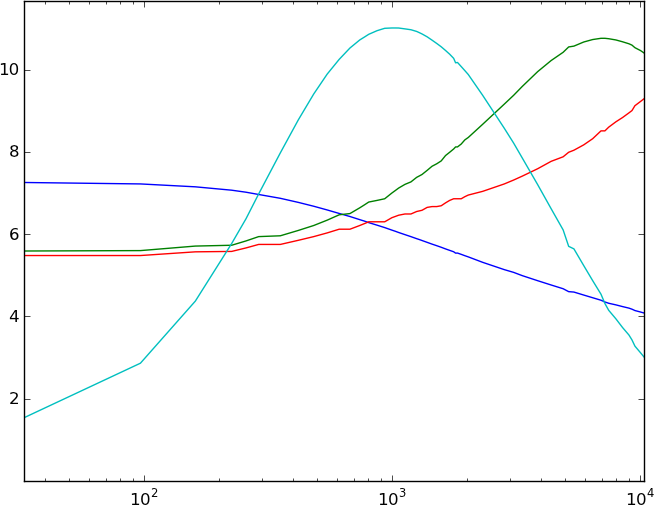
\includegraphics[width=84mm]{Figures/model/L1544model_used.png}
 \label{fig:l1544_model}
 \caption{Model of the pre-stellar core L1544 used as the envelope of the young protoplanetary disk in the hybrid model. Showing temperature (red) and dust (green) temperature in kelvin, log number density (blue) in cm$^{-3}$ and inward velocity$\times$100 (cyan) in m$\,$s$^{-1}$. Adapted from Keto \& Caselli (2010) and Keto et al. (2012, in preparation).}
\end{figure}

\begin{figure*}
 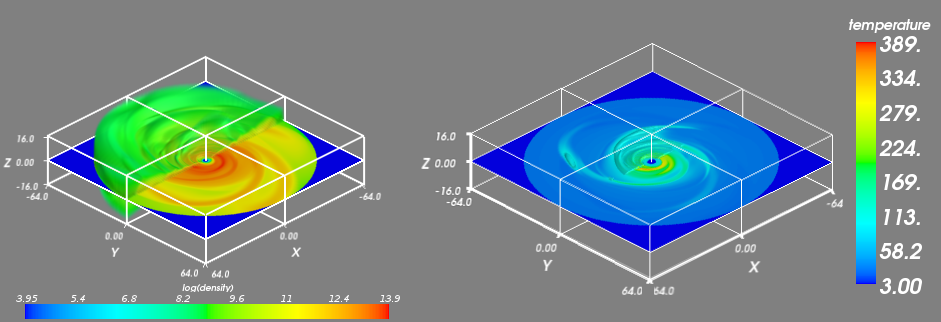
\includegraphics[width=168mm]{Figures/model/rhoT2.png}
 \label{rhoT} 
 \caption{Left: A 3D plot of log number density (m$^{-3}$) showing the spiral structure in the xy plane and scale height of the disc. Right: The 3D temperature structure of the disc; regions cooler than 40 degrees are not shown in 3D, demonstrating the narrow central region containing hot material.}
\end{figure*}

\begin{figure*}
 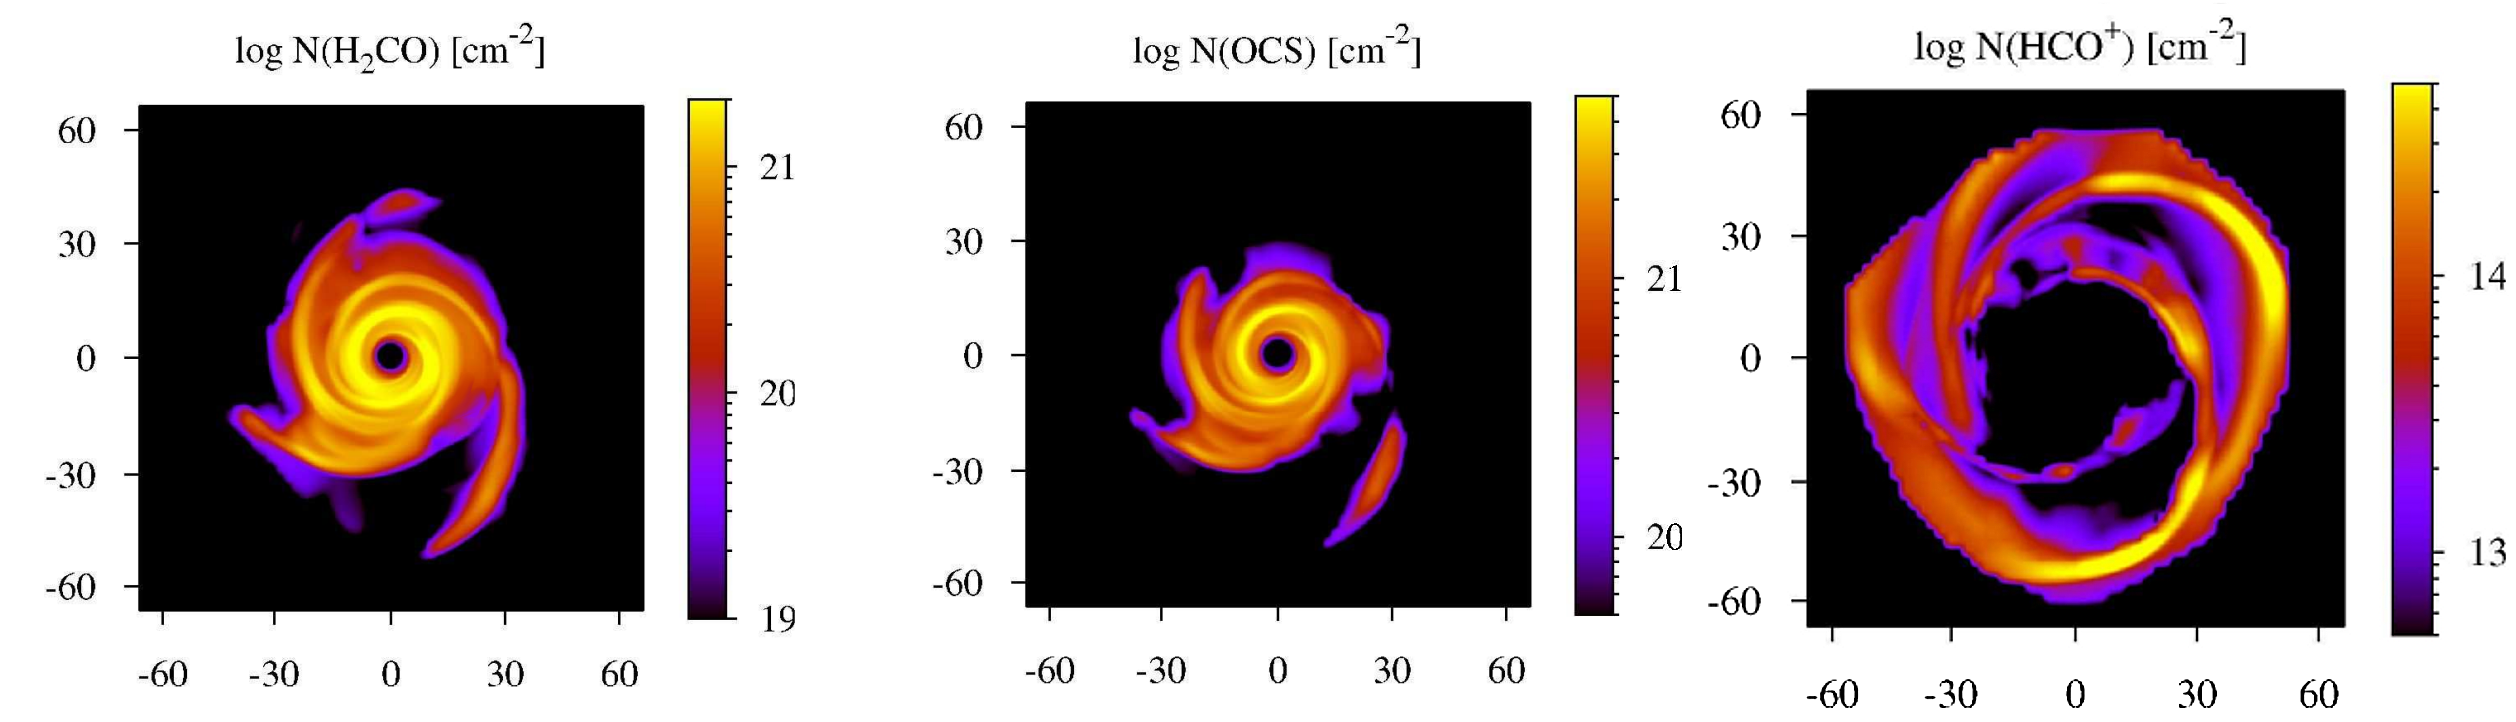
\includegraphics[width=168mm]{Figures/model/columnDensities2.png}
 \label{Chemistry} 
 \caption{Column densities of H$_2$CO, OCS and HCO$^+$ used in the disc model. Figure adapted from Ilee at al. (2011)}
\end{figure*}

\begin{figure}
 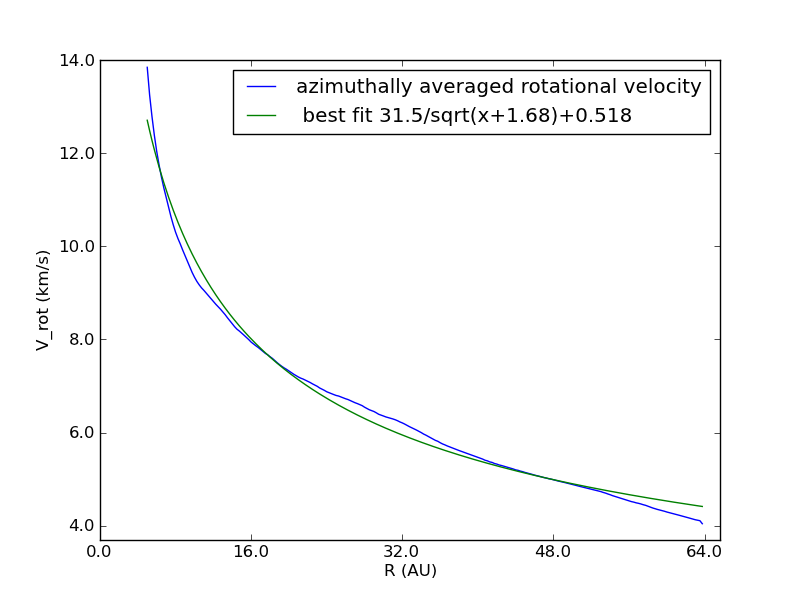
\includegraphics[width=84mm]{Figures/model/rotational_velocities.png}
 \label{velocity}
 \caption{Azimuthaly averaged rotational velocity in the disc mid-plane with best fit curve}
\end{figure}


%-describe the physical structure of the disk (density and temperature) -- one figure showing the physical structure and the kinematics (2-panels figure)
The pre-stellar core structure is maintained down to a radius of 80\,AU, within which the young protoplanetary disk has been plugged in. The disk structure is derived by the hydrodynamic model of Boley(2007) and Boley (2009). The particular model considered here (as well as in Ilee et al. 2011) is a 0.39$\,\rm{M}_\odot$ self-gravitating disc featuring prominent spiral arms. H$_2$ number densities in the disc range from 10$^{10}$-10$^{19}\,\rm{m}^{-3}$, and temperatures range from 30-400 K (figure \ref{rhoT}). The dust and gas temperatures in the disc are assumed to be in equilibrium. The model is sampled over a regular grid of size 256$\times$256$\times$64 with spatial resolution of 0.5$\,$au in x, y and z. The gas/dust mass ratio was assumed to be 1/100 throughout both sections model and the opacities were given by the model of dust grains with thick icy mantles and 10$^6\,$yr coagulation from Ossenkopf and Henning (1994). THe gas number density and temperature structure are displayed in Fig. XX. \newline

%The majority of the mass lies in the mid-plane of the disc. For the models using a smoothed disc the same physical and chemical model is used but with the temperature, density and abundance averaged in $\phi$. The gas/dust mass ratio was assumed to be 1/100 throughout both sections model and the opacities were given by the model of dust grains with thick icy mantles and 10$^6\,$yr coagulation from Ossenkopf and Henning (1994)\newline

%-describe the chemistry  - refer to Ilee et al. which have been taken as input to the rad transfer (RT) code
Chemical abundances in the disc were taken from Ilee et. al (2011) which followed the changes of chemical abundances of trace particles moving through the disc as it evolved. The abundances of 125 species related by 1334 reactions were followed through the time evolution of the disc. These abundances were interpolated onto a 51$^3$ grid covering the disc with cells of size 2.2$\times$2.2$\times$0.22$\,$au.  Fig. XX shows a sample of column density maps from Ilee et al. (2011), pointing out the different regions traced by H$_2$CO and OCS, which mostly probe the central warm regions, and HCO$^+$, which preferentially trace the outer spiral pattern as in the central region is destroyed by water molecules (see Ilee et al. 2011 for details).   The simple chemistry in the KC2010 model, adopted here as the envelope of the protoplanetary disk, does not provide detailed abundances of molecular species (besides CO and H$_2$O, see also Caselli et al. 2012). As discussed in the result section (Sec.\,\ref{sec:model_results}), rough guesses have been made based on values measured toward similar object. 

%NOTE: WE SHOULD TALK ABOUT THESE SPECIES AFTER WE SHOW WHICH SPECIES WE SELECT FOR THE RADIATIVE TRANSFER. 
%Abundances in the envelope model were as follows:\newline

%(tableify this?)
%HCO$^+$: As the H$_2$O profile from Caselli et al. (2012, submitted) scaled so that the maximum abundance is 10$^{-8}$\newline
%HNO: Constant abundance of 5$\times$10$^{-11}$\newline
%HCS$^+$: Constant abundance of 10$^{-11}$\newline
%OCS: Constant abundance of 10$^{-9}$\newline
%H$_2$CO: 1.5$\times$10$^{-9}$ decreased by a factor of 40 at radii less than 8250au (Young et al 2004)\newline
%CS:  3$\times$10$^{-9}$ decreased by a factor of 10,000 at radii less than 6700au (Tafalla, santiago-garcia and myers 2006)\newline
%CO: As the H2O profile from Caselli (2012, submitted) scaled so that the maximum abundance is CO maximum ***which is....***\newline


\subsection{The radiative transfer code} \label{subsec:radiative_transfer_code}
%-describe the RT used (LIME) 
The radiative transfer program used, LIME (Brinch \&Hogerheijde 2010), calculates line intensities based on a weighted sample of randomly chosen points in a continuous 3D model. The method of selecting these points is given in the griding section (NOTE: WHERE IS THE GRIDING SECTION?). At each of these points, the density of the main collision partner (H$_2$), gas and dust temperatures, velocity, molecular abundances and turbulent velocity are taken from the model. These points are then smoothed by Lloyds algorithm (Lloyd 1982) in order to minimise the variation in distance between points whilst keeping the same underlying distribution. These points are then connected by Delaunay triangulation (NOTE: YOU NEED TO EXPLAIN THIS - MAYBE IN A FOOTNOTE) and it is down these paths that photon propagation is restricted (figures \ref{grid}). The level populations of the selected molecules are calculated at each of these points from collisional and radiative (de)excitation and the local radiation field is calculated. This is repeated 20 times with the populations of each level converging towards a single value.\newline


\begin{figure}
 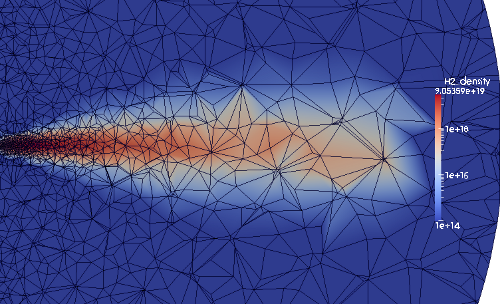
\includegraphics[width=84mm]{Figures/model/Lime_grid3.png}
 \label{grid}
 \caption{A plot of the points selected by the griding process and the paths down which photons can propagate overlaid on a smoothed density model. The points are more concentrated at small radii and in the densest regions.}
\end{figure}

\begin{figure}
 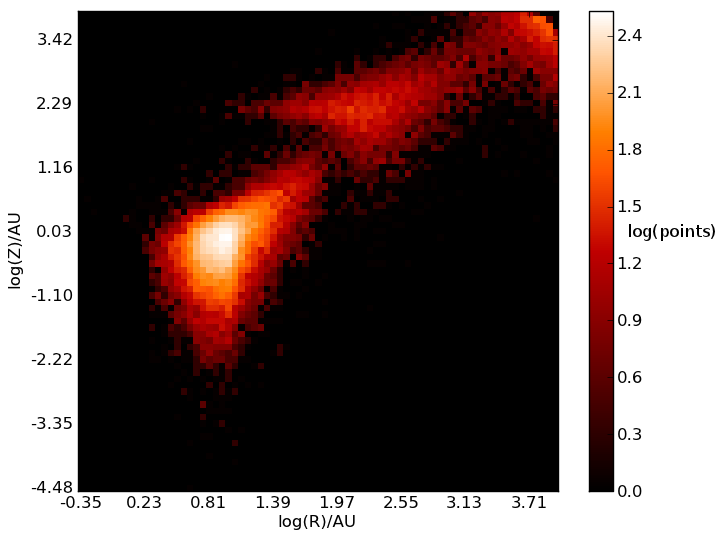
\includegraphics[width=84mm]{Figures/model/lime_points_rz_histo.png}
 \label{points}
 \caption{A histogram of the point distribution throughout the model.}
\end{figure}

In order to construct the grid, points are randomly selected from the volume, then compared against a reference point (NOTE: WHAT IS THE COMPARISON FOR?). Grid points are selected at random in cylindrical co-ordinates, linearly spaced in z and $\phi$ and logarithmically spaced in r. For each point to be selected, a random number $\alpha$ is drawn from the semi-open set [0,$\,$1) as a threshold. After selection of random co-ordinates, the hydrogen density and molecular density at the point (n and m, respectively) are compared against the densities of a reference point on the inner edge of the disc (n$_0$ and m$_0$). If $\alpha<\left( \frac{n}{n_0} \right)^{0.3}$ or $\alpha< \left( \frac{m}{m_0} \right)^{0.3}$ then the point is selected for use, if not then another r, $\phi$, z co-ordinate is selected. The weighting function and griding functions (NOTE: CAN YOU PLEASE EXPLAIN WHAT A GRIDING FUNCTION IS?) were selected empirically to sample all the scales while ensuring that the majority of points are located into the inner disc (where the density is higher --IS THIS LAST STATEMENT, WHICH I JUST ADDED, CORRECT?). 20\% of these points are forced to be at radii greater than $\sqrt{R_{min}R_{max}}$ (where $R_{min}$ and $R_{max}$ are the inner and outer radius of the model) in order to stop too many of the selecected points clustering in the high density disc and leaving the envelope undersampled. In addiation to this method of selection, 5\% of the points are linearly distributed in x, y and z with no bias with regards to density or abundance. This provides a minimum level of sampling for the large low density regions in the outer parts of the simulated volume. See figure \ref{points} for example of the points distribution in r, z. \newline

\begin{figure}
 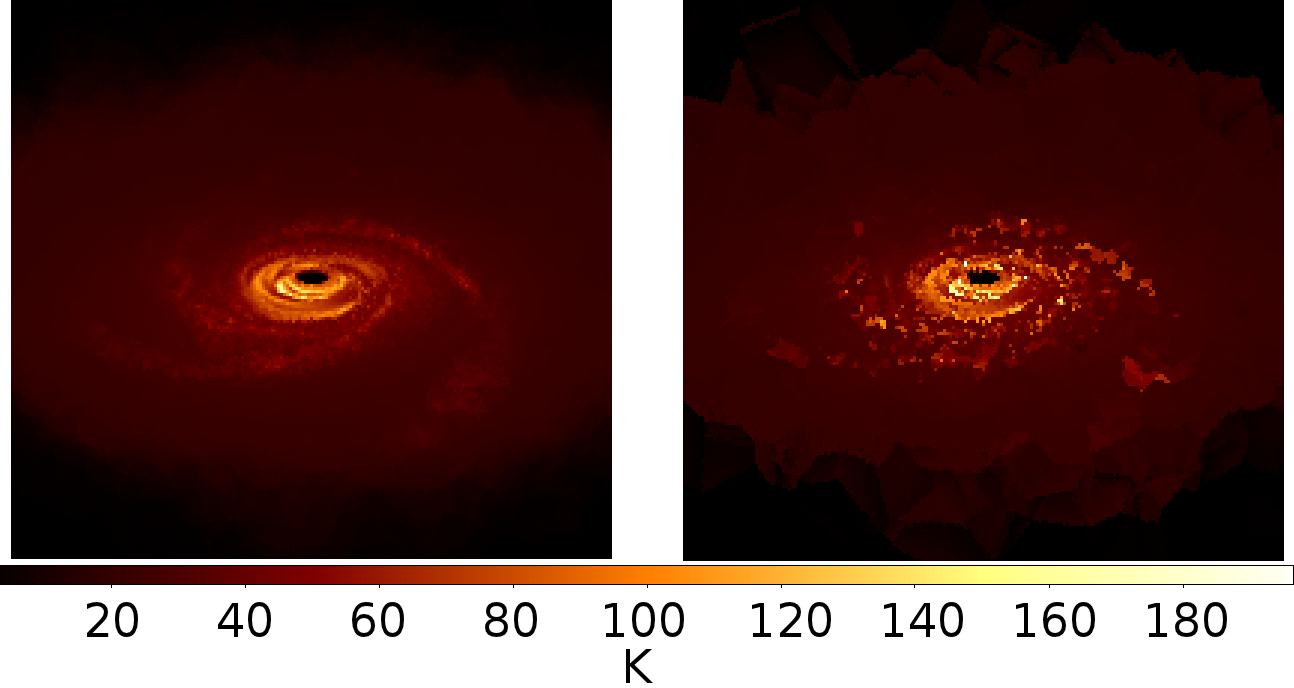
\includegraphics[width=84mm]{Figures/sim/average_comparison.png}
 \label{averages}
 \caption{A plot showing the difference between a single LIME continuum image at 300$\,$GHz (right) and the average of ten such images from different runs of the same model in LIME (left).}
\end{figure}


\section{Model Results} \label{sec:model_results}

NOTE: YOU NEED TO ADD A LITTLE HISTORY ON WHY YOU SELECTED THESE SPECIES TO DO THE RADIATIVE TRANSFER. CAN YOU PLEASE RESTRUCTURE THIS SECTION ?
%Figures showing the RT results in a few molecules/transitions (CO, HCO$^+$, HCN, OCS, H2CO, NH3 --- maybe H2O,H2$^{18}$O [to try first])
The results of these simulations for the molecules OCS, HCO$^+$, H$_2$CO and isotopologues of CO are shown here, other molecules simulated but not shown include HCN, HNC, HNO, HCS$^+$ and  CS.
For the purpose of simulating observations the model was placed at roughly the distance of nearby low-mass star forming regions (100$\,$pc) and is inclined 30$^\circ$ to edge on. From these observations integrated intensity, intensity weighted velocity and position velocity diagrams through the centre of the model were created.
The simulations done are focused upon frequencies within ALMA band 7, selected to give the best trade off between resolution and sensitivity for early ALMA science.
(Note the moment 1 and 0 maps were created by integrating between -12.5 to -0.5 km$\,$s$^{-1}$ and +0.5 to +12.5 km$\,$s$^{-1}$ to avoid being dominated by the contribution from the envelope, this can be seen in some PV diagrams as the strong absorption feature at all positions around zero velocity, moment 1 maps are shown with a cutoff of 1/1000 of the peak emission/absorption value)\newline

\begin{figure}
 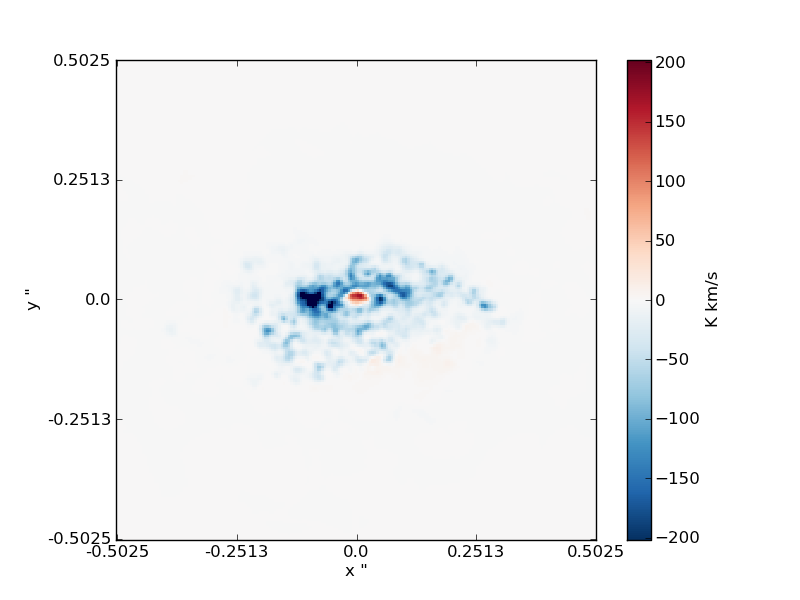
\includegraphics[width=84mm]{Figures/sim/imageCO_3-2_30deg_contSub.png}

 \caption{CO J=3-2 Continuum subtracted mom0}
\end{figure}

\begin{figure}
 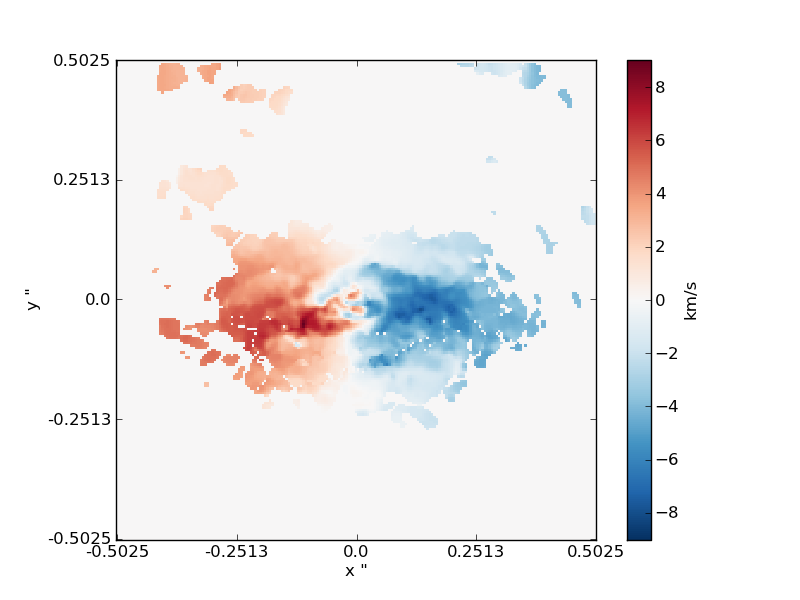
\includegraphics[width=84mm]{Figures/sim/imageCO_3-2_30deg_mom1.png}

 \caption{CO J=3-2 moment 1 map}
\end{figure}

\begin{figure}
 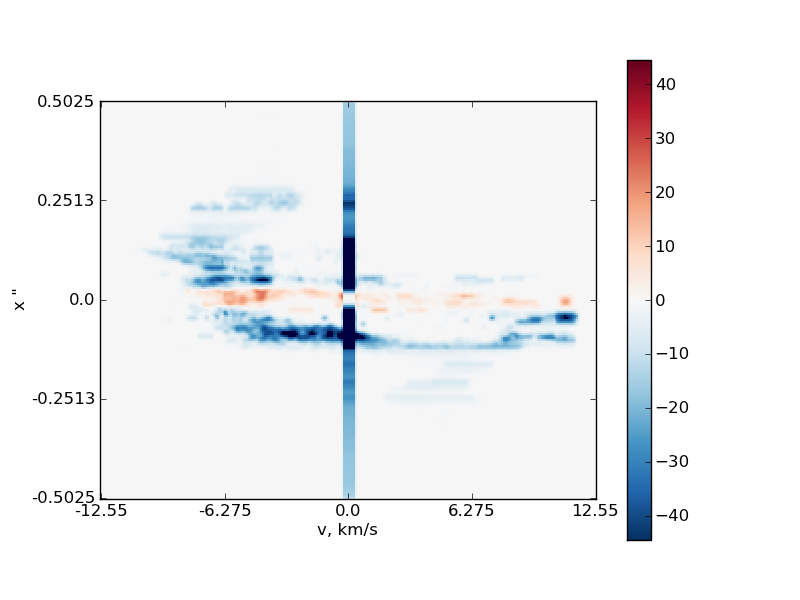
\includegraphics[width=84mm]{Figures/sim/imageCO_3-2_30deg_PV_centre.png}

 \caption{CO J=3-2 PV through y=0''}
\end{figure}

Figures 6,7 and 8 show synthetic images of the CO J=3-2 line at 345.8$\,$GHz. As the upper level for this line is at 33$\,$K above the ground state this transition should be excited through out disc. given the large and uniform nature of the abundance of CO in the disc this line will be optically thick and this is only mapping the outer regions of the disc. In common with most transitions simulated, the line is seen almost exclusively in absorption against the disc continuum. The region of emission in the centre is where there is no continuum background to be absorbed.  Some indications of spiral structure can be seen but are indistinct. ***not sure how useful these are, might be worth cutting them?***\newline



\begin{figure}
 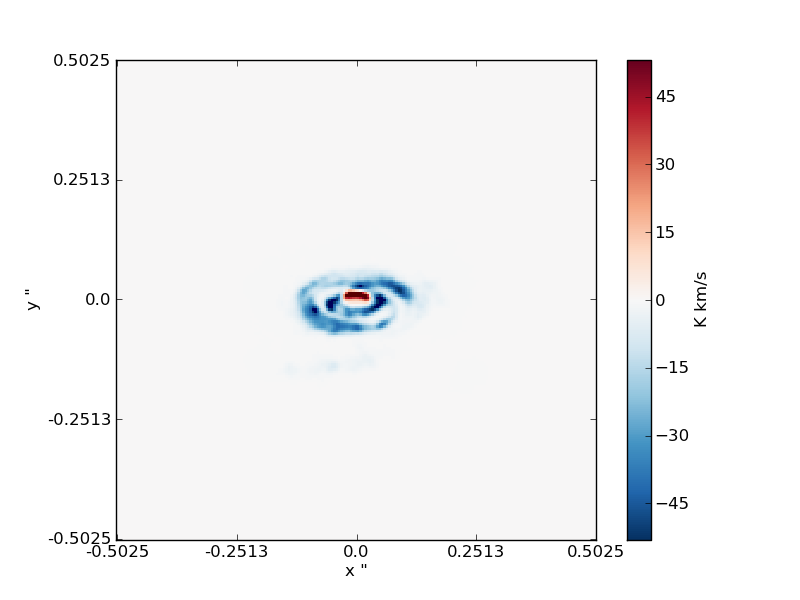
\includegraphics[width=84mm]{Figures/sim/imageOCS_28-27_30deg_composite_contSub.png}
 \label{OCS_mom0}
 \caption{OCS 28-27 Continuum subtracted mom0}
\end{figure}

\begin{figure}
 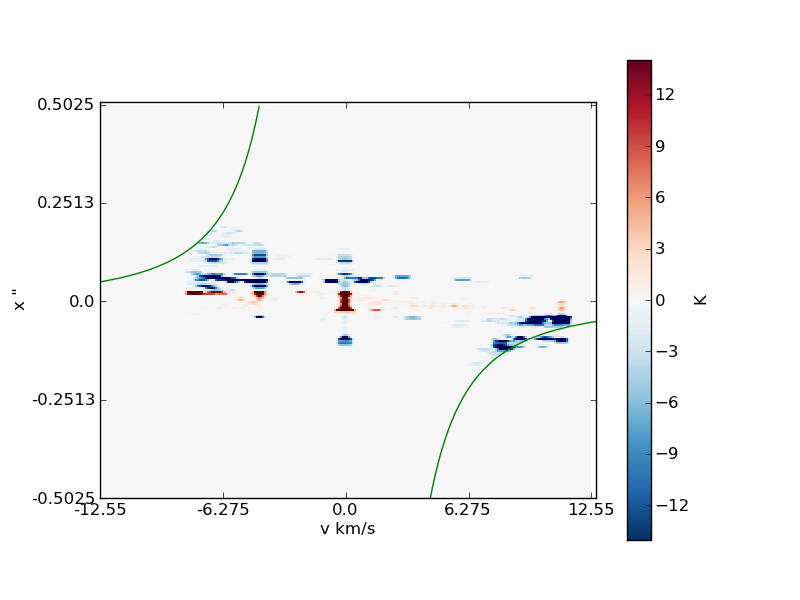
\includegraphics[width=84mm]{Figures/sim/imageOCS_28-27_30deg_composite_PV_centre.png}

 \caption{OCS 28-27 PV through centre}
\end{figure}

After looking at a variety of lines which could be observed of ALMA band 6 or 7 (211-275$\,$GHz and 275-373$\,$GHz) we found that the OCS lines in alma band 7 (22-21 through 30-29) with upper energy levels between 161 and 271 K above the ground state provide a way to trace hot shocked gas in spiral arms without resolving structure. Figures \ref{OCS_mom0} \& \ref{smoothOCS_mom0} show the integrated intensity of the OCS J=28-27 line in the model described previously and one where the disc section of the model is an axis-symmetric model created by taking the azimuthal average of density, temperature and molecular abundance. The order of magnitude difference in the line intensity provides a method to detect hot dense gas without being able to resolve the spiral structure spatially.\newline

\begin{figure}
 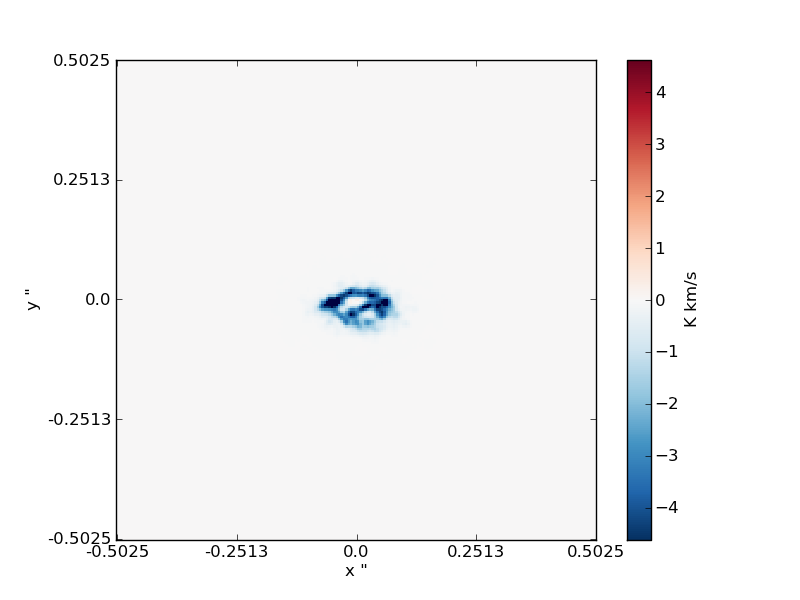
\includegraphics[width=84mm]{Figures/sim/imagesmoothedOCS_28-27_30deg_contSub.png}
 \label{smoothOCS_mom0}
 \caption{SmoothedOCS 28-27 Continuum subtracted mom0}
\end{figure}


 
%\begin{figure}
% 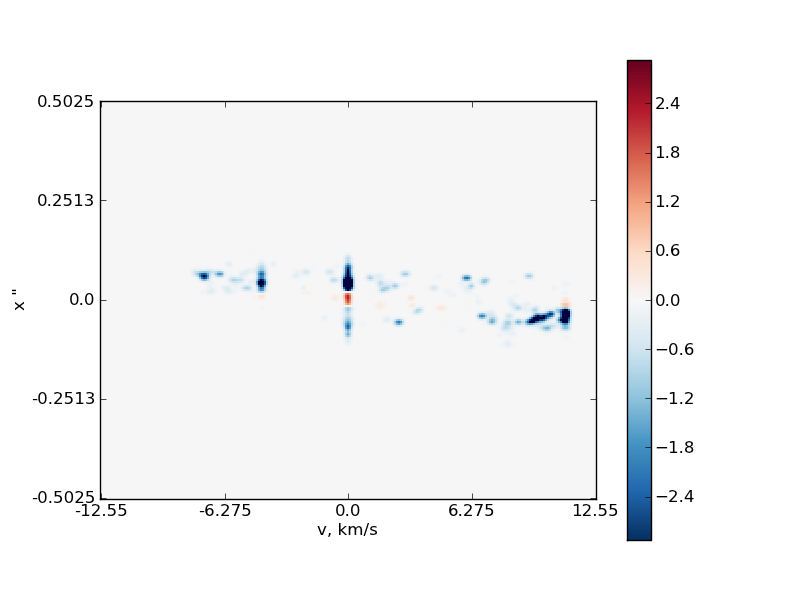
\includegraphics[width=84mm]{Figures/sim/imagesmoothedOCS_28-27_30deg_PV_centre.png}
%
% \caption{SmoothedOCS 28-27 PV through centre}
%\end{figure}

\begin{figure}
 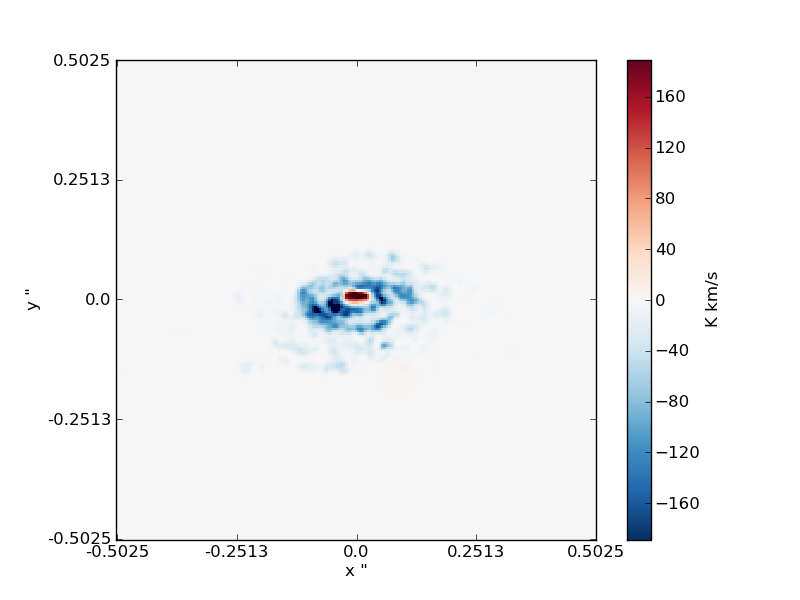
\includegraphics[width=84mm]{Figures/sim/imageH2CO_4-0-4->3-0-3_30deg_contSub.png}

 \caption{H$_2$CO 4$\,$0$\,$4 - 3$\,$0$\,$3 Continuum subtracted mom0}
\end{figure}

\begin{figure}
 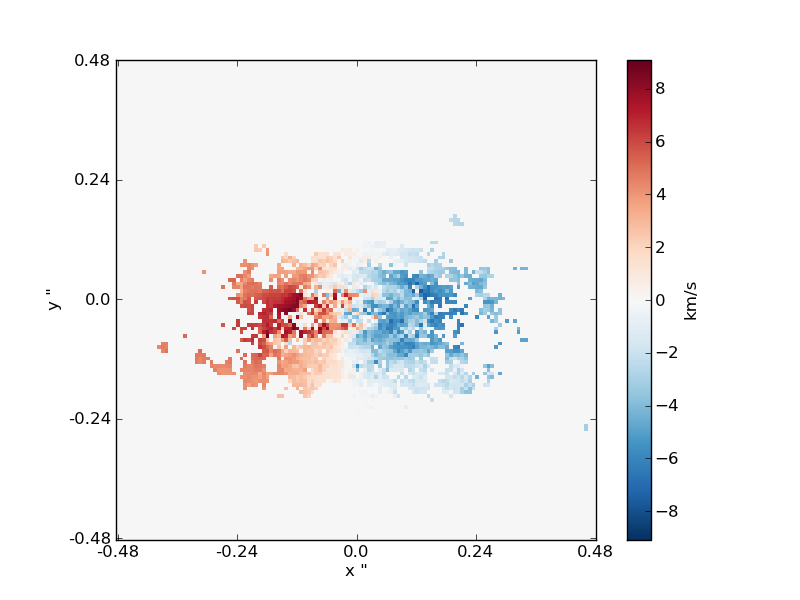
\includegraphics[width=84mm]{Figures/sim/imageH2CO_4-0-4->3-0-3_30deg_mom1.png}

 \caption{H$_2$CO 4$\,$0$\,$4 - 3$\,$0$\,$3 PV through centre}
\end{figure}

\begin{figure}
 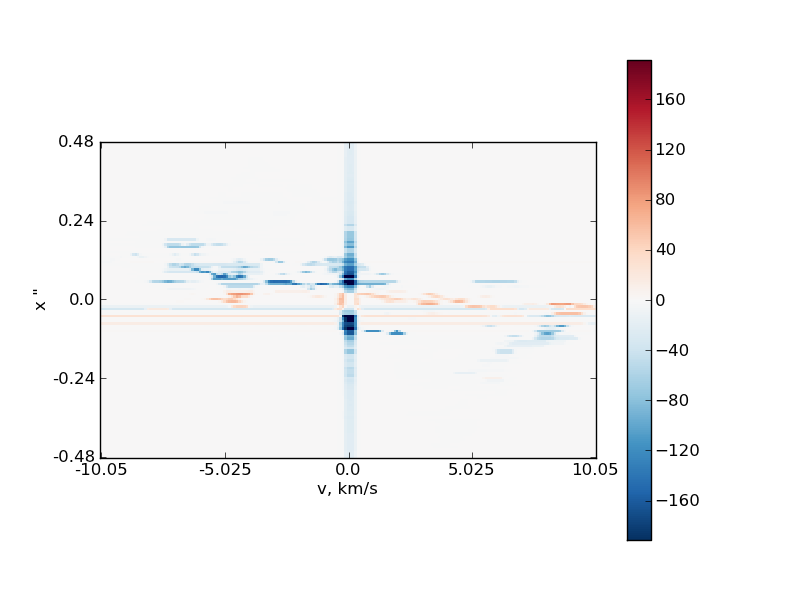
\includegraphics[width=84mm]{Figures/sim/imageH2CO_4-0-4->3-0-3_30deg_PV_centre.png}

 \caption{H$_2$CO 4$\,$0$\,$4 - 3$\,$0$\,$3 PV through centre}
\end{figure}

More complex molecules such as H$_2$CO with many closely spaced spectral lines can be used to gain an estimate on the temperature of a region. 

(figure of temperature as a function of line ratio for 2 sets of formaldehyde lines and map of derived temperature, talk to P about this. This doesn't seem doable with the lines around 1mm for alma)\newline

\begin{figure}
 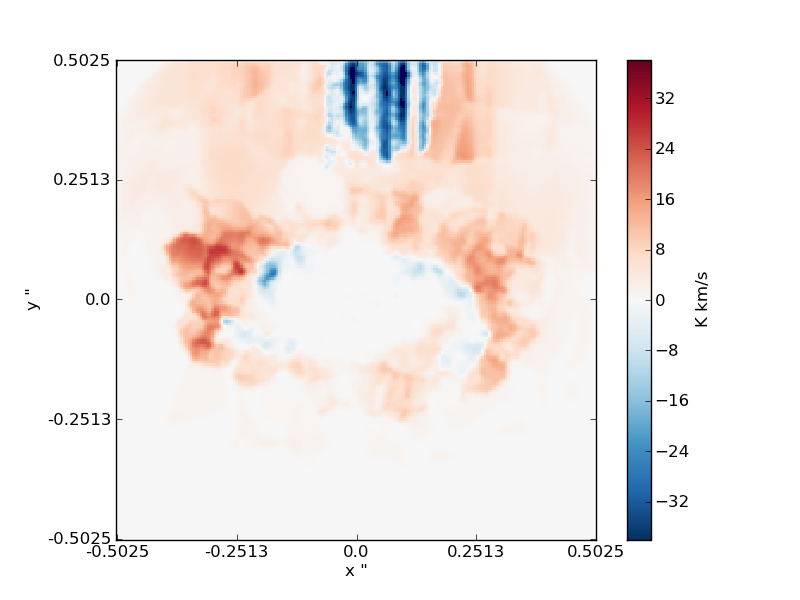
\includegraphics[width=84mm]{Figures/sim/imageHCOp_1-0_30deg_contSub.png}

 \caption{HCO$^+$ 1-0 Continuum subtracted mom0}
\end{figure}

\begin{figure}
 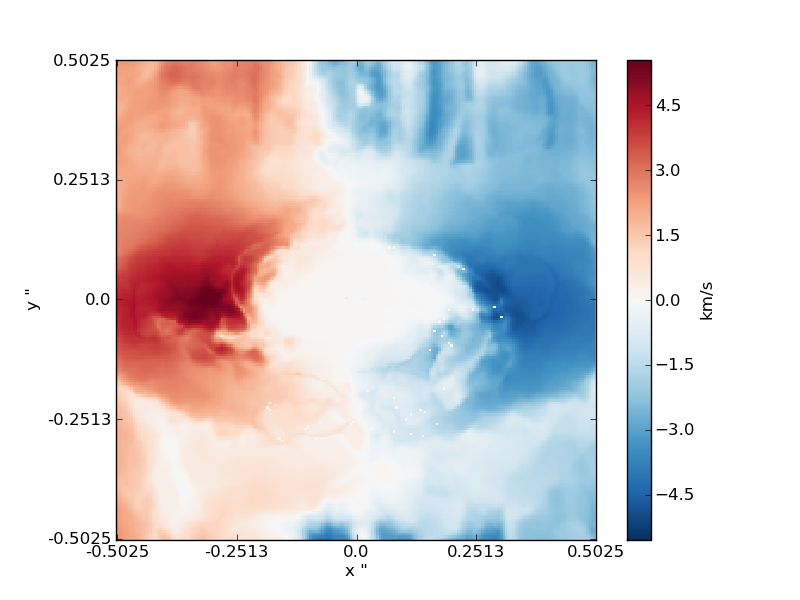
\includegraphics[width=84mm]{Figures/sim/imageHCOp_1-0_30deg_mom1.png}

 \caption{HCO$^+$ 1-0 mom1map}
\end{figure}

\begin{figure}
 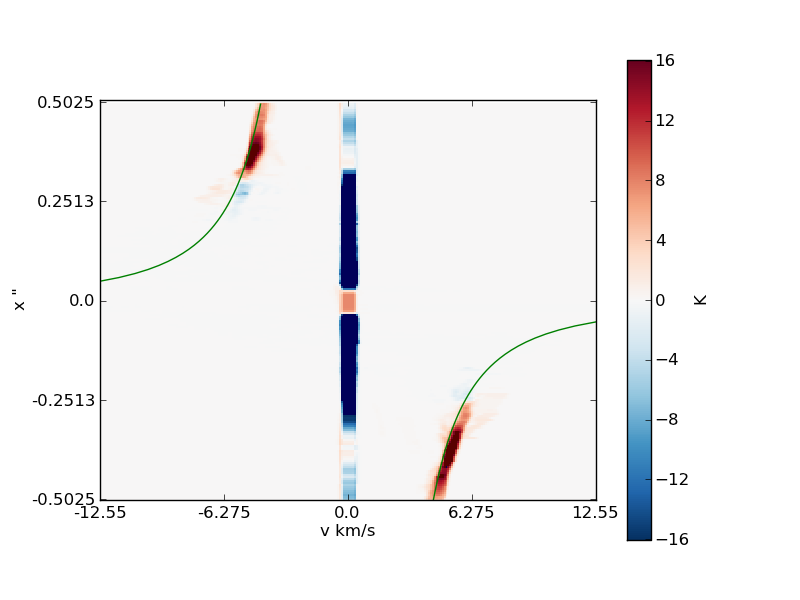
\includegraphics[width=84mm]{Figures/sim/imageHCOp_1-0_30deg_PV_centre.png}

 \caption{HCO$^+$ 1-0 pv through centre}
\end{figure}

\begin{figure}
 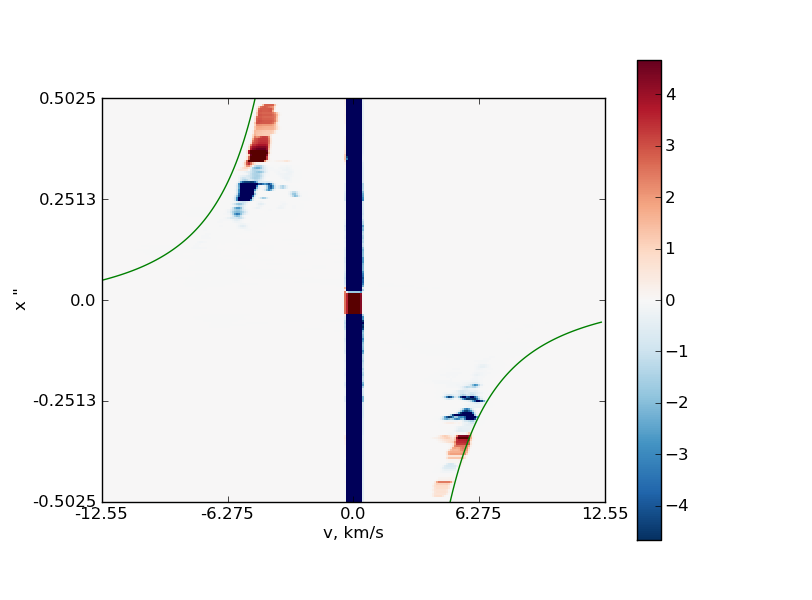
\includegraphics[width=84mm]{Figures/sim/imageHCOp_3-2_30deg_PV_centre_2.png}
 \label{hcop_pv}
 \caption{HCO$^+$ 3-2 PV through centre with rotation curve from figure \ref{velocity} *** should the velocities in this be reduced by cos(30) as we're not in the plane of rotation? ***}
\end{figure}

Some molecules such as HCO$^+$ trace only the outer regions of the disc (Ilee 2011) and so can be used to look at the extended velocity and physical structure. In these colder less dense regions we see the molecular lines in emission rather than absorption. Figure \ref{hcop_pv} shows the rotation curve of the model as shown in figure \ref{velocity} against the HCO$^+$ J=3-2 line emission. It is clear that from observations such as these the rotation curve of a disc could be reconstructed.\newline
\newline



In all the simulations except HCO$^+$ we see molecular lines in absorption throughout the majority of the disc and in some cases a small amount of emission towards the centre, where the inclination of the disc allows us the view the low density but moderate temperature region inside the inner edge of the spiral structures without any high temperature and density material behind it.\newline




\section{ALMA Predictions} \label{sec:alma_predictions}

%- current status (Cycle 1) - Figure
%OCS + C18O + H2CO + HNO/CS/
%- final status - Figure 


\begin{figure}
 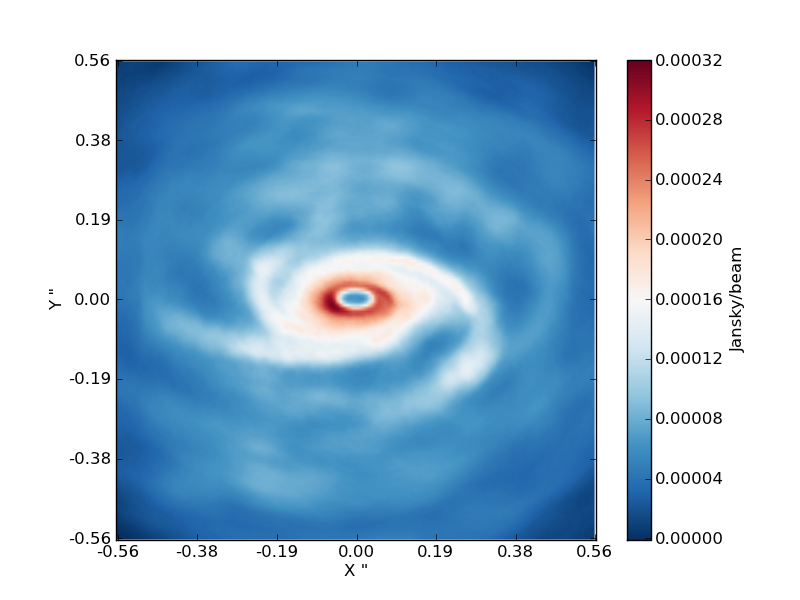
\includegraphics[width=84mm]{Figures/sim/casa_cont_337GHz.png}

 \caption{continuum emission at 337GHz simulated for ALMA most extended configuration}
\end{figure}

\begin{figure}
 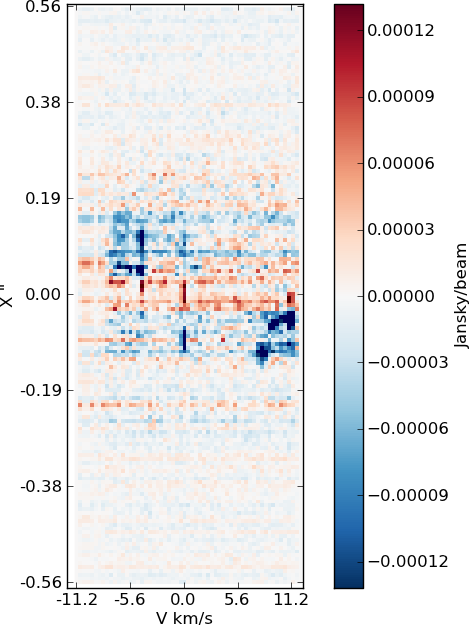
\includegraphics[width=54mm]{Figures/sim/casa_OCS_28-27_pv.png}

 \caption{OCS 28-29 pv diagram simulated for ALMA most extended configuration}
\end{figure}


\begin{figure}
 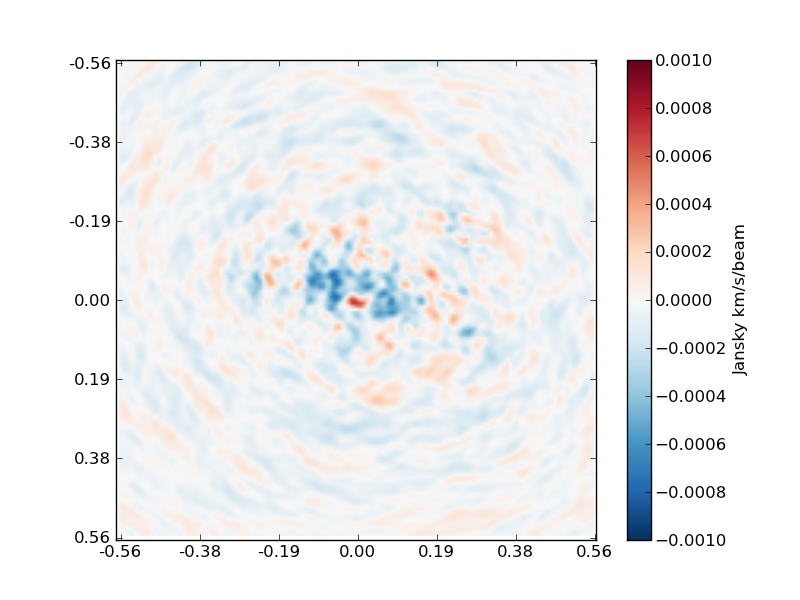
\includegraphics[width=84mm]{Figures/sim/casa_OCS_28-27_mom0.png}

 \caption{OCS 28-29 integrated intesity simulated for ALMA most extended configuration}
\end{figure}


\begin{figure}
 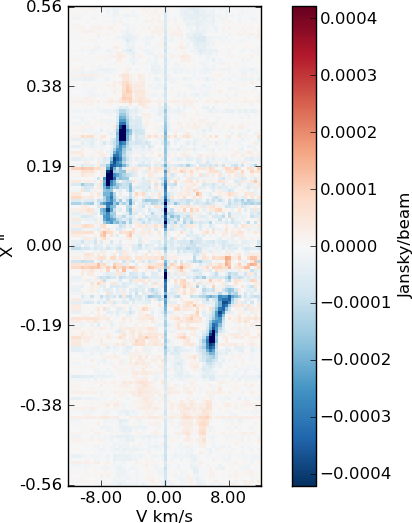
\includegraphics[width=54mm]{Figures/sim/casa_C17O_3-2_pv.png}

 \caption{C17O 3-2 30 deg PV through centre simulated for ALMA most extended configuration}
\end{figure}

\begin{figure}
 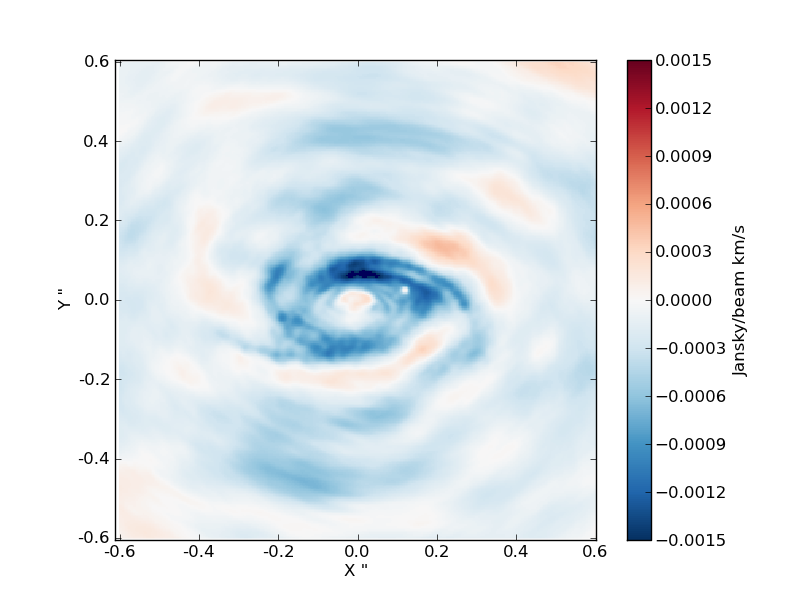
\includegraphics[width=84mm]{Figures/sim/casa_C17O_3-2_mom0.png}

 \caption{C17O 3-2 30 deg integrated intensity simulated for ALMA most extended configuration}
\end{figure}




\section{Discussion and conclusions} \label{sec:discussion}

In this paper we have performed radiative transfer simulations of a hybrid model comprising a 0.4$\, M_\odot$ self gravitating disc with radius 64$\,AU$ showing spiral density waves, surrounded by an envelope simulated as a collapsing 10$\,M_\odot$ BE-sphere. CASA simulations show that at a distance of 100$\,$pc both spatial resolution of the spirals in such a disc and extraction of kinematic and temperature from molecular lines are possible in ALMA band 7. Our simulations show that many  molecular species are predominantly seen in absorption towards the centre of  self-gravitating protoplanetary discs. The quiescent nature of the envelope around such discs only obscures them within $\pm\,0.5 km\,s^{-1}$.\newline
Hot, shocked gas can be detected in such a disc without resolving it by observing OCS transitions between 26-27 to 30-29.\newline
One assumption made in this model is that the gas and dust are in thermal equilibrium.If they are not and the dust is significantly cooler than the gas then transitions may not show up in absorption.\newline
The mass of the disc used (0.4$\,\rm{M}_\odot$) is on the high end for early discs (citations for estimate of early class 1 disc masses).\newline 
In the model spirals shock heat the mid-plane layer and the colder more diffuse gas absorbs the continuum from it, this results in molecular lines being seen in absorbtion whenever lines of sight pass through the cold diffuse gas at larger heights on to the hot dense midplane of the disc. Rotation curves can be gathered from these observations even with spiral structure\newline




\section*{Acknowledgements}

stuff here
\newpage


\appendix

\section[]{Other Inclinations}

Figures showing different inclinations  
\begin{figure}
 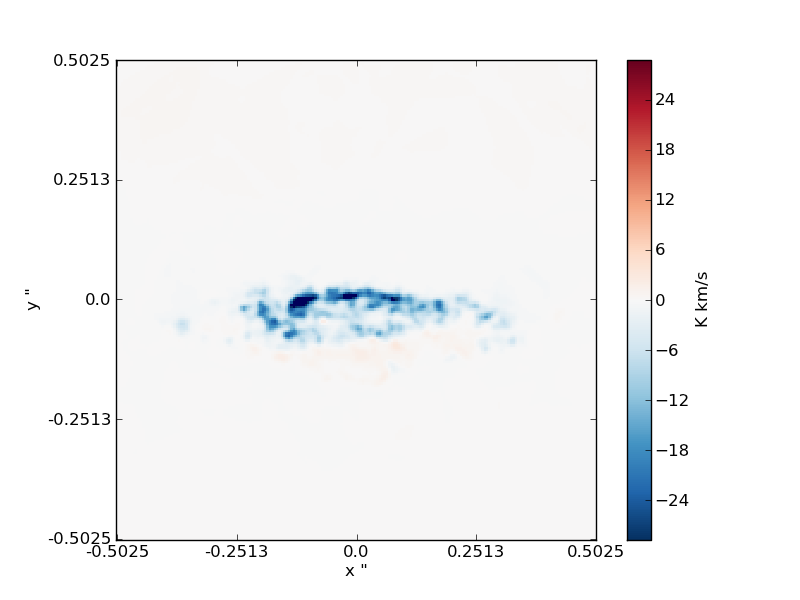
\includegraphics[width=84mm]{Figures/sim/imageC18O_3-2_15deg_contSub.png}

 \caption{C18O 3-2 15 deg Continuum subtracted mom0}
\end{figure}

%\begin{figure}
% 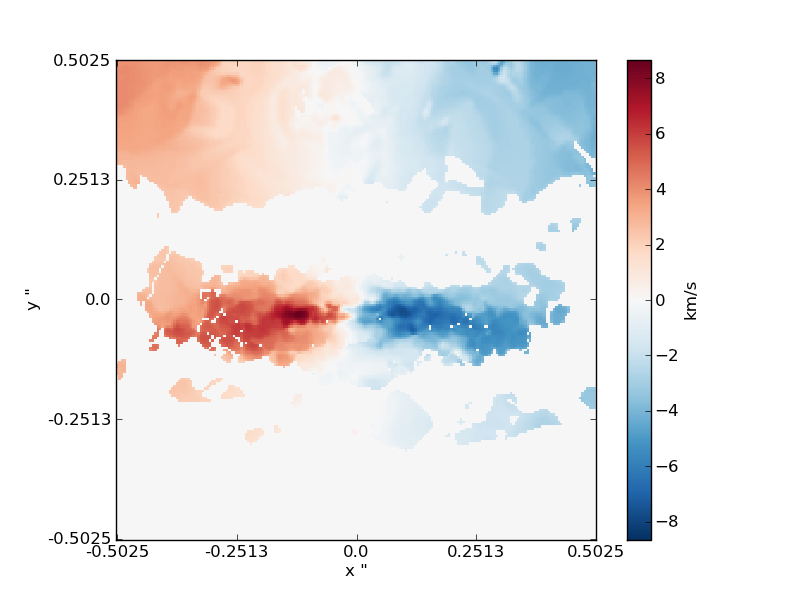
\includegraphics[width=84mm]{Figures/sim/imageC18O_3-2_15deg_mom1.png}
%
% \caption{C18O 3-2 15 deg mom1map}
%\end{figure}

\begin{figure}
 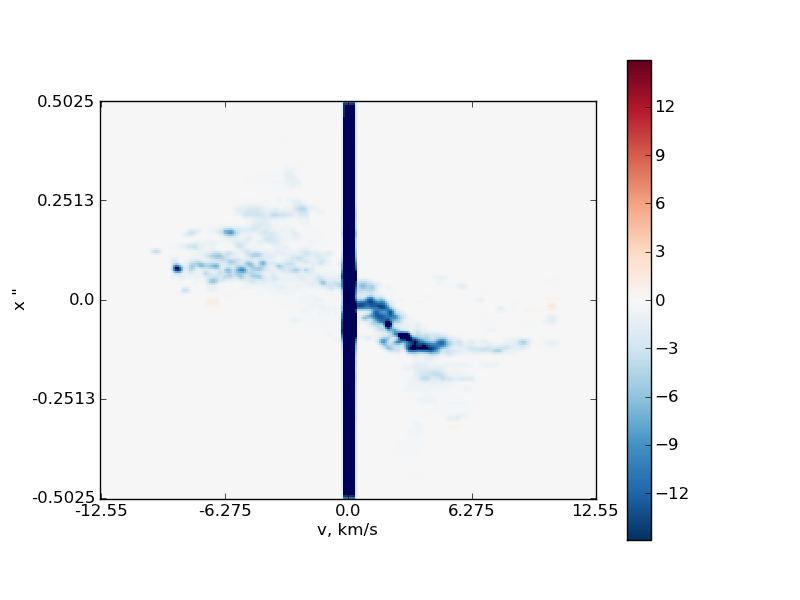
\includegraphics[width=84mm]{Figures/sim/imageC18O_3-2_15deg_PV_centre.png}

 \caption{C18O 3-2 PV 15 deg through centre}
\end{figure}


\begin{figure}
 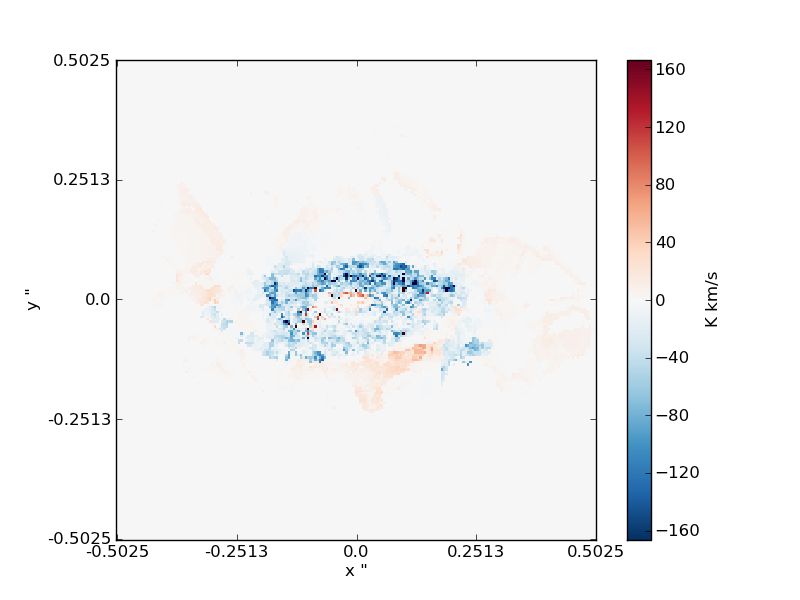
\includegraphics[width=84mm]{Figures/sim/imageC18O_3-2_30deg_contSub.png}

 \caption{C18O 3-2  30 deg Continuum subtracted mom0}
\end{figure}




%\begin{figure}
% 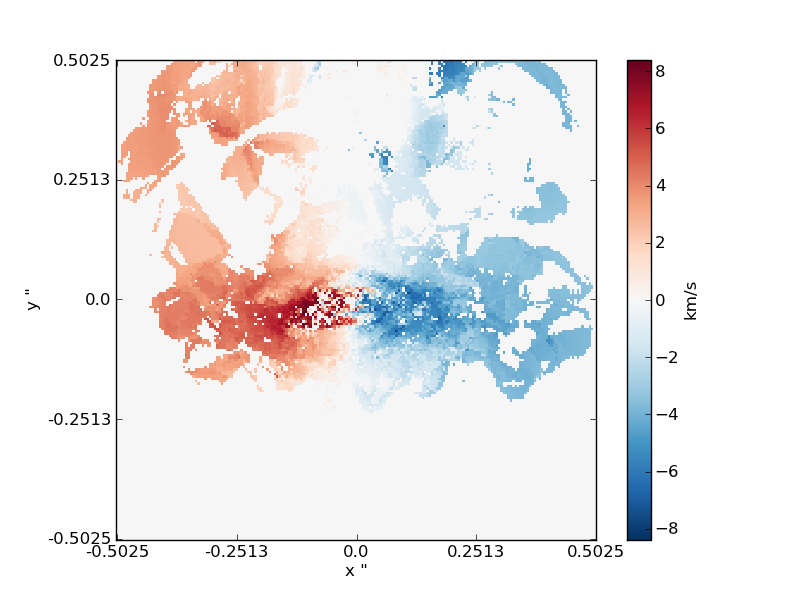
\includegraphics[width=84mm]{Figures/sim/imageC18O_3-2_30deg_mom1.png}
%
% \caption{C18O 3-2 30 deg mom1map}
%\end{figure}

\begin{figure}
 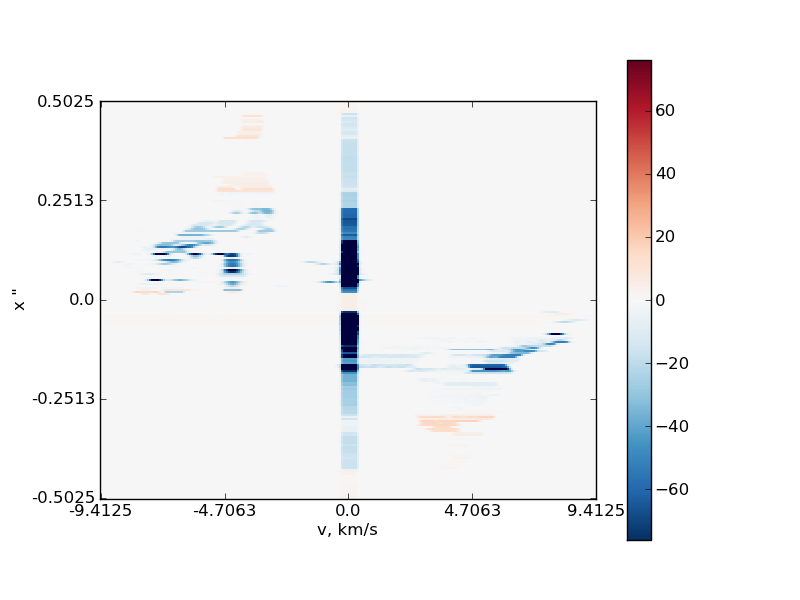
\includegraphics[width=84mm]{Figures/sim/imageC18O_3-2_30deg_PV_centre.png}

 \caption{C18O 3-2 30 deg PV through centre}
\end{figure}

\begin{figure}
 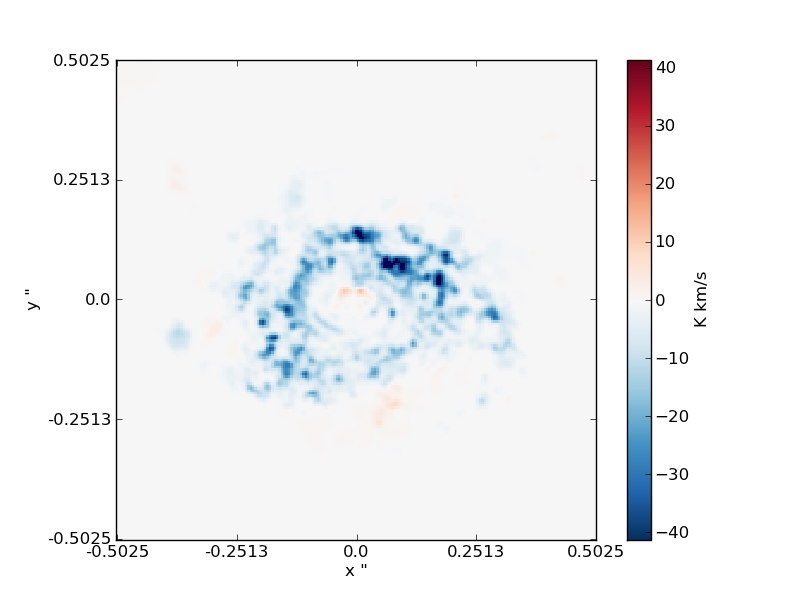
\includegraphics[width=84mm]{Figures/sim/imageC18O_3-2_45deg_contSub.png}

 \caption{C18O 3-2 45 deg Continuum subtracted mom0}
\end{figure}

%\begin{figure}
% 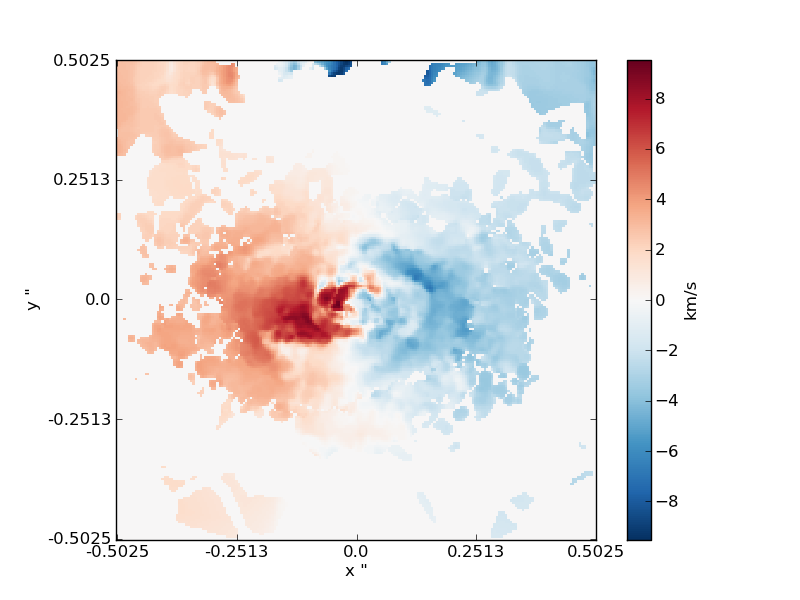
\includegraphics[width=84mm]{Figures/sim/imageC18O_3-2_45deg_mom1.png}
%
% \caption{C18O 3-2 45 deg mom1map}
%\end{figure}

\begin{figure}
 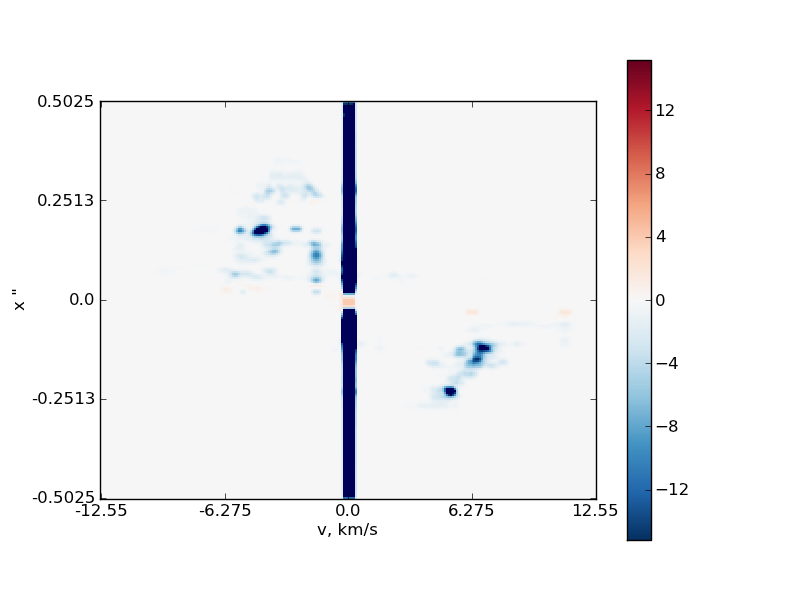
\includegraphics[width=84mm]{Figures/sim/imageC18O_3-2_45deg_PV_centre.png}

 \caption{C18O 3-2 45 deg PV through centre}
\end{figure}


\begin{figure}
 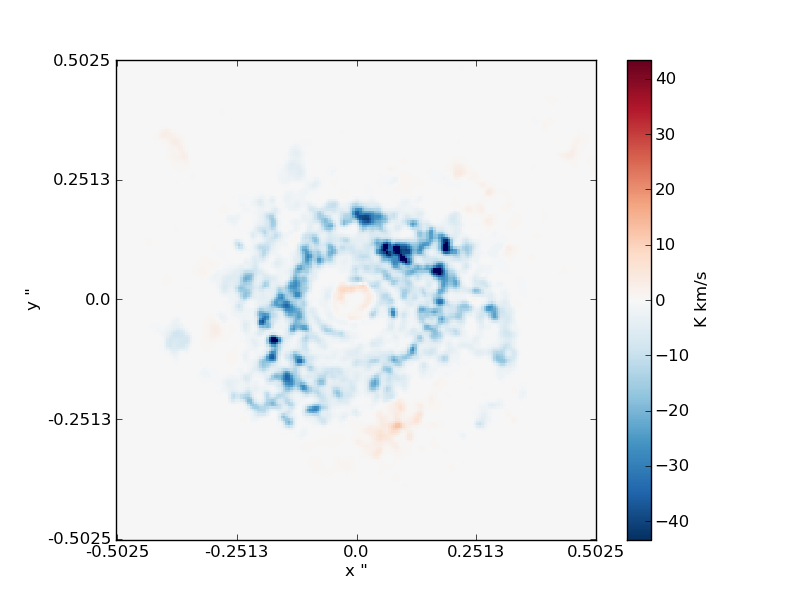
\includegraphics[width=84mm]{Figures/sim/imageC18O_3-2_60deg_contSub.png}

 \caption{C18O 3-2 60 deg Continuum subtracted mom0}
\end{figure}

%\begin{figure}
% 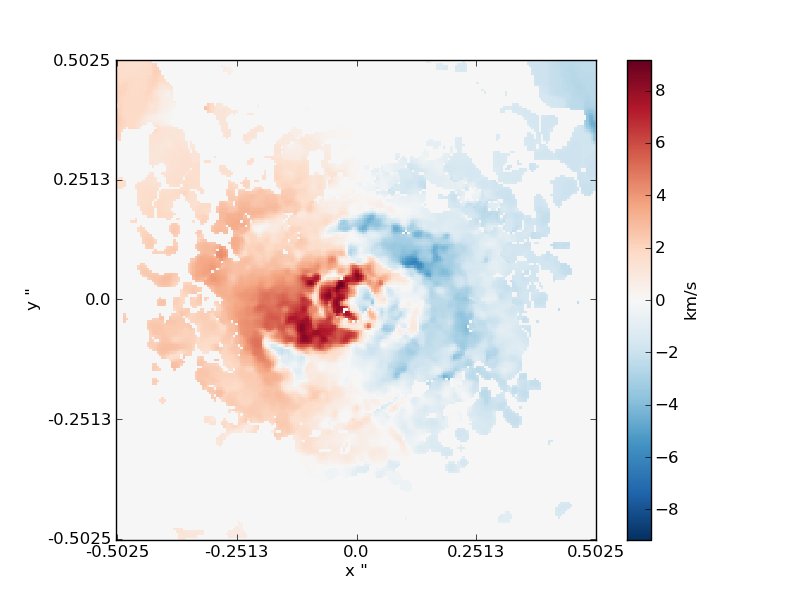
\includegraphics[width=84mm]{Figures/sim/imageC18O_3-2_60deg_mom1.png}
%
% \caption{C18O 3-2 60 deg mom1map}
%\end{figure}

\begin{figure}
 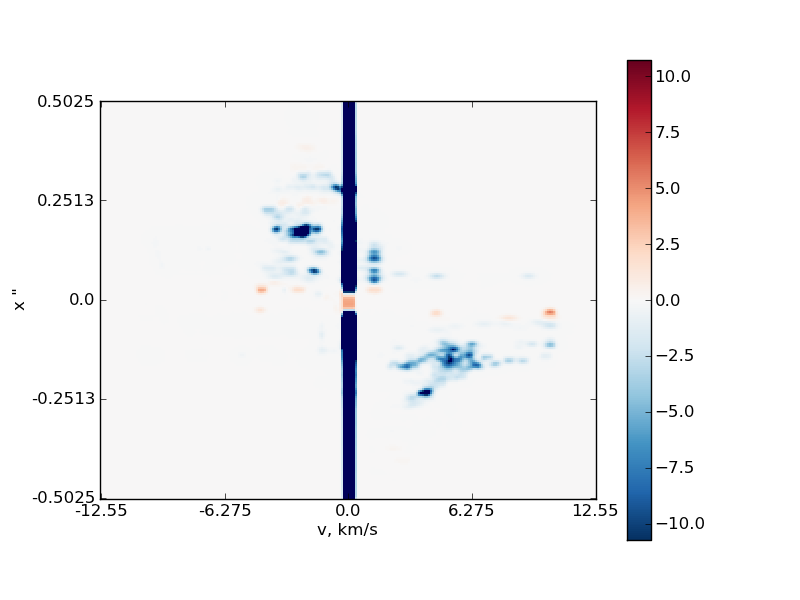
\includegraphics[width=84mm]{Figures/sim/imageC18O_3-2_60deg_PV_centre.png}

 \caption{C18O 3-2 60 deg PV through centre}
\end{figure}

\begin{figure}
 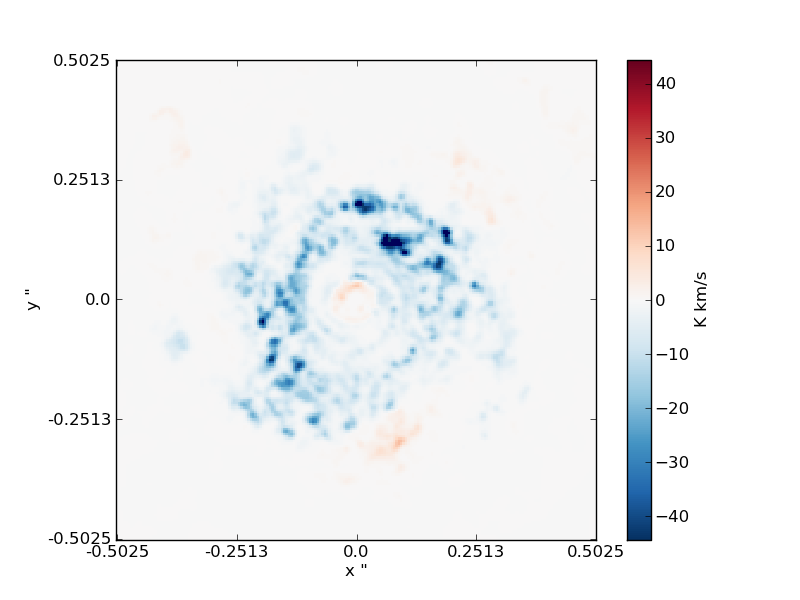
\includegraphics[width=84mm]{Figures/sim/imageC18O_3-2_75deg_contSub.png}

 \caption{C18O 3-2 75 deg Continuum subtracted mom0}
\end{figure}

%\begin{figure}
% 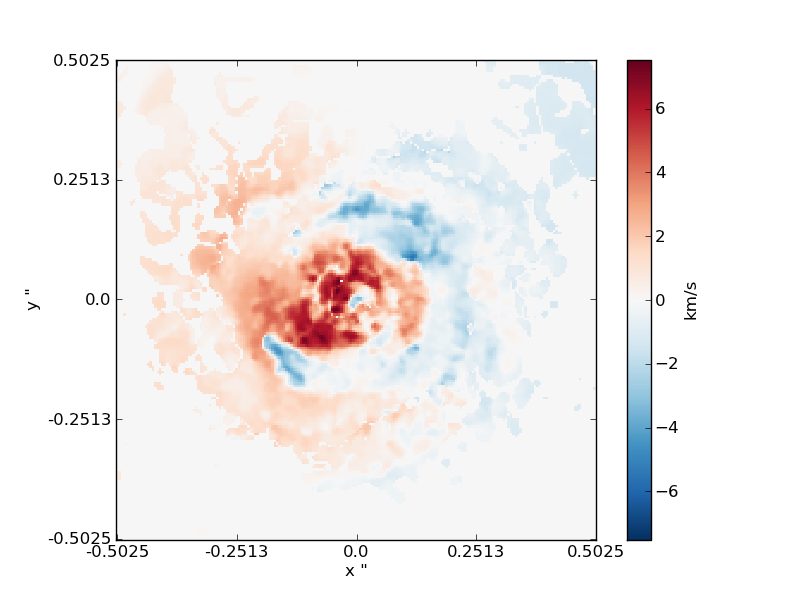
\includegraphics[width=84mm]{Figures/sim/imageC18O_3-2_75deg_mom1.png}
%
% \caption{C18O 3-2 75 deg mom1map}
%\end{figure}

\begin{figure}
 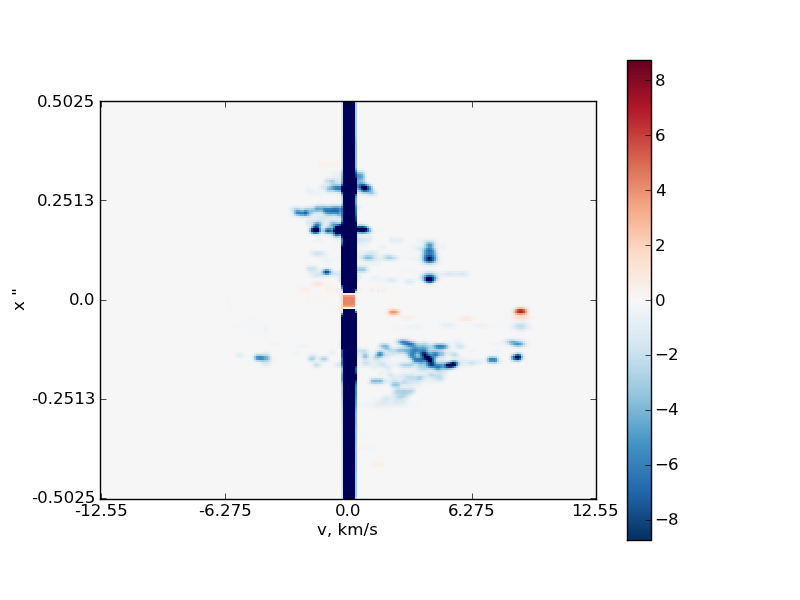
\includegraphics[width=84mm]{Figures/sim/imageC18O_3-2_75deg_PV_centre.png}

 \caption{C18O 3-2 75 deg PV through centre}
\end{figure}

%
%(This appendix was not part of the original paper by
%A.V.~Raveendran and is included here just for illustrative
%purposes. The references are not relevant to the text of the
%appendix, they are references from the bibliography used to
%illustrate text before and after citations.)
%
%Spectroscopic observations of bright quasars show that the mean
%number density of Ly$\alpha$ forest lines, which satisfy certain
%criteria, evolves like $\rmn{d}N/\rmn{d}z=A(1+z)^\gamma$, where
%$A$ and~$\gamma$ are two constants.  Given the above intrinsic
%line distribution we examine the probability of finding large gaps
%in the Ly$\alpha$ forests.  We concentrate here only on the
%statistics and neglect all observational complications such as the
%line blending effect \citep[see][for example]{b11}.
%
%Suppose we have observed a Ly$\alpha$ forest between redshifts $z_1$
%and~$z_2$ and found $N-1$ lines.  For high-redshift quasars $z_2$~is
%usually the emission redshift $z_{\rmn{em}}$ and $z_1$ is set to
%$(\lambda_{\rmn{Ly}\beta}/\lambda_{\rmn{Ly}\alpha})(1+z_{\rmn{em}})=0.844
%(1+z_{\rmn{em}})$ to avoid contamination by Ly$\beta$ lines.  We
%want to know whether the largest gaps observed in the forest are
%significantly inconsistent with the above line distribution.  To do
%this we introduce a new variable~$x$:
%%
%\begin{equation}
%x={(1+z)^{\gamma+1}-(1+z_1)^{\gamma+1} \over
%     (1+z_2)^{\gamma+1}-(1+z_1)^{\gamma+1}}.
%\end{equation}
%%
%$x$ varies from 0 to 1.  We then have $\rmn{d}N/\rmn{d}x=\lambda$, where $\lambda$
%is the mean number of lines between $z_1$ and $z_2$ and is given by
%%
%\begin{equation}
%\lambda\equiv{A[(1+z_2)^{\gamma+1}-(1+z_1)^{\gamma+1}]\over\gamma+1}.
%\end{equation}
%%
%This means that the Ly$\alpha$ forest lines are uniformly
%distributed in~$x$. The probability of finding $N-1$ lines between $z_1$
%and~$z_2$, $P_{N-1}$, is assumed to be the Poisson distribution.
%%
%\newpage
%%
%\begin{figure}
%\vspace{11pc}
%\caption{$P(>x_{\rmn{gap}})$ as a function of $x_{\rmn{gap}}$ for,
% from left to right, $N=160$, 150, 140, 110, 100, 90, 50, 45 and~40.
% Compare this with \protect\citet{b15}.}
%\label{appenfig}
%\end{figure}
%
%\subsection{Subsection title}
%
%We plot in Fig.~\ref{appenfig} $P(>x_{\rmn{gap}})$ for several $N$
%values. We see that, for $N=100$ and $x_{\rmn{gap}}=0.06$,
%$P(>0.06)\approx20$ per cent.  This means that the probability of
%finding a gap with a size larger than six times the mean
%separation is not significantly small. When the mean number of
%lines is large, $\lambda\sim N>>1$, our $P(>x_{\rmn{gap}})$
%approaches the result obtained by \citet[fig. 4]{b22} for small
%(but still very large if measured in units of the mean separation)
%$x_{\rmn{gap}}$, i.e., $P(>x_{\rmn{gap}})\sim N(1-
%x_{\rmn{gap}})^{N-1}\sim N {\rmn{exp}}(-\lambda x_{\rmn{gap}})$.
%
\bsp
%
\label{lastpage}
%
\end{document}
